\subsection{UML Diagram}
\begin{enumerate}
    \item UML Diagram 1 \\
    \hspace{1cm} This UML Diagram dictates the authentic login by different users, user search  by using username and management of the user profiles.
    \vspace{1cm}
    \begin{center}
        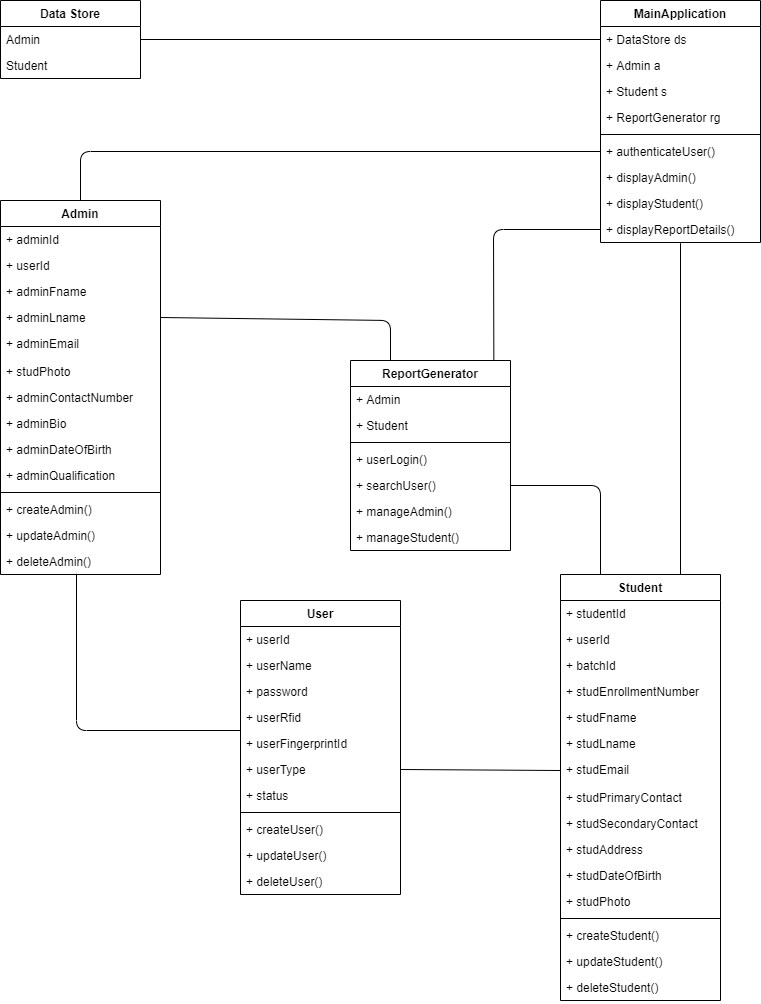
\includegraphics[scale=.5]{Images/uml/Profile_manage.png}
    \end{center}

    \newpage
    \item UML Diagram 2 \\
    \hspace{1cm} This UML dictates the management of different Batches and Courses, and users can view the information regarding batches and courses.
    \vspace{1cm}
    \begin{center}
        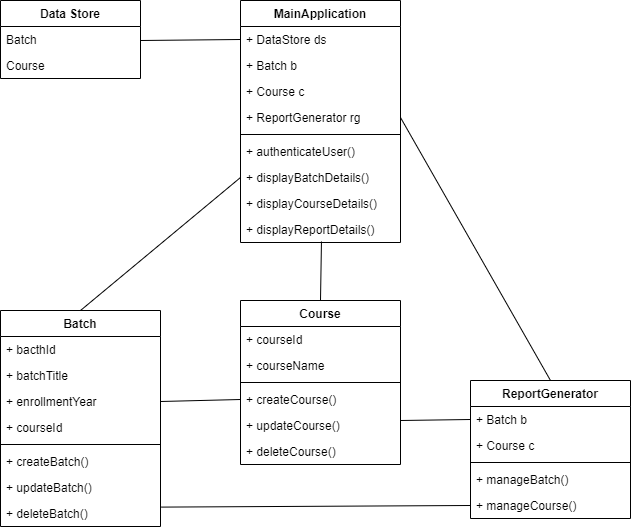
\includegraphics[scale=.5]{Images/uml/Batch_Course_manage.png}
    \end{center}
       
    \newpage
    \item UML Diagram 3 \\
    \hspace{1cm} This UML dictates the management of different Semesters and Semesters of particular batches, and the intended user can view these informations.
    \vspace{1cm}
    \begin{center}
        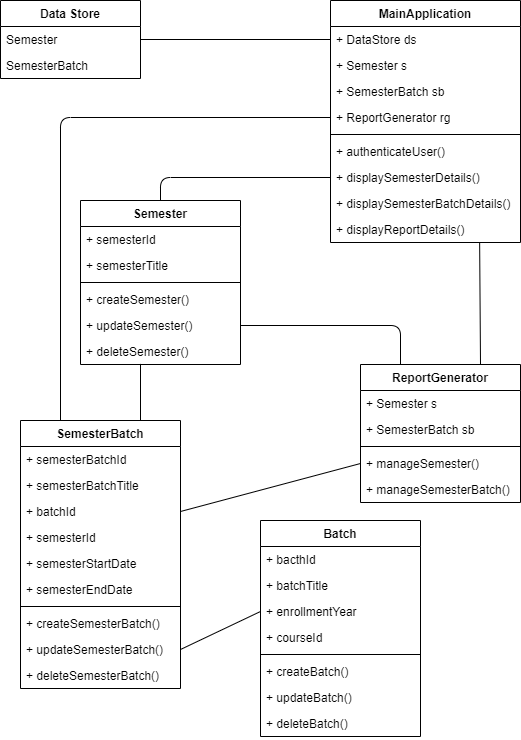
\includegraphics[scale=.5]{Images/uml/Semester_Batch_manage.png}
    \end{center}

    \newpage
    \item UML Diagram 4 \\
    \hspace{1cm} This UML dictates the management of different Subject, syllabus, topics and subtopics, and intended users can view the syllabus.
    \vspace{1cm}
    \begin{center}
        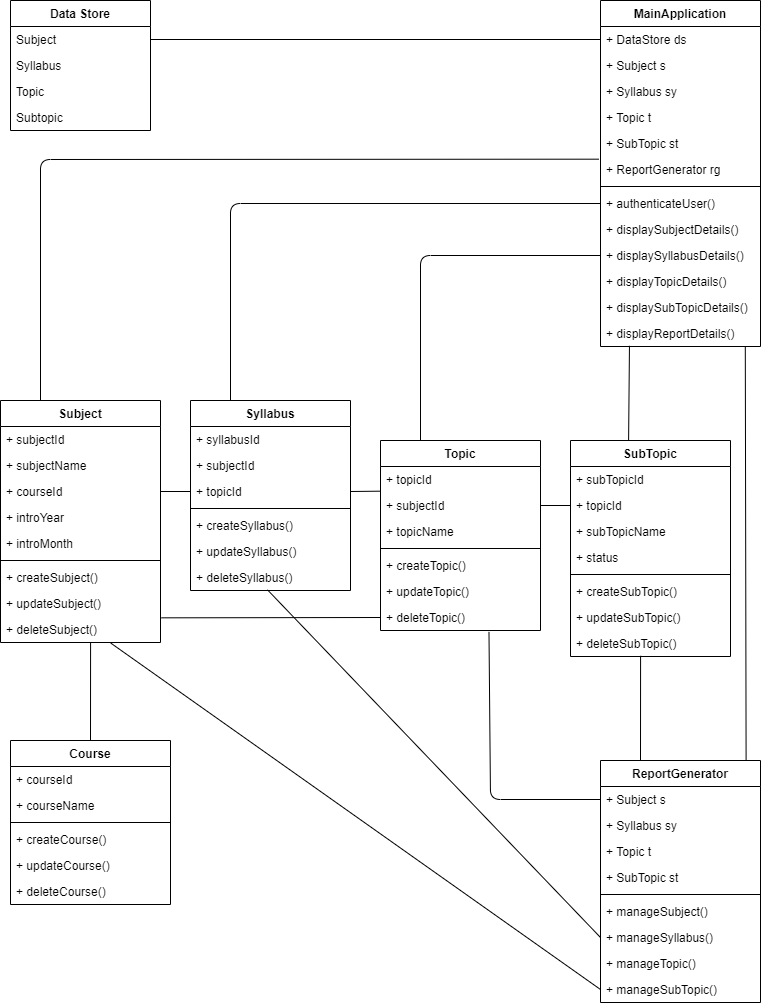
\includegraphics[scale=.5]{Images/uml/Subject_Syllabus_manage.png}
    \end{center}
    
    \newpage
    \item UML Diagram 5 \\
    \hspace{1cm} This UML dictates the management of lecture schedules, intended users can view the daily lecture schedules.
    \vspace{1cm}
    \begin{center}
        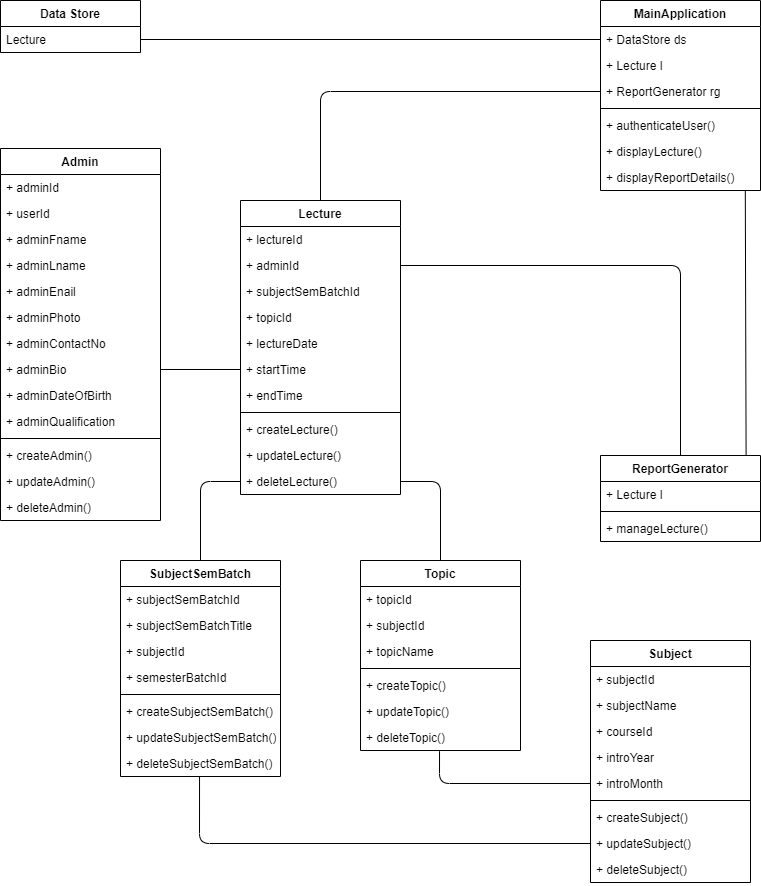
\includegraphics[scale=.5]{Images/uml/Lecture_manage.png}
    \end{center}
    
    \newpage
    \item UML Diagram 6 \\
    \hspace{1cm} This UML dictates the management of attendance, intended user can mark the attendance and view the attendance details of students.
    \vspace{1cm}
    \vspace{1cm}
    \begin{center}
        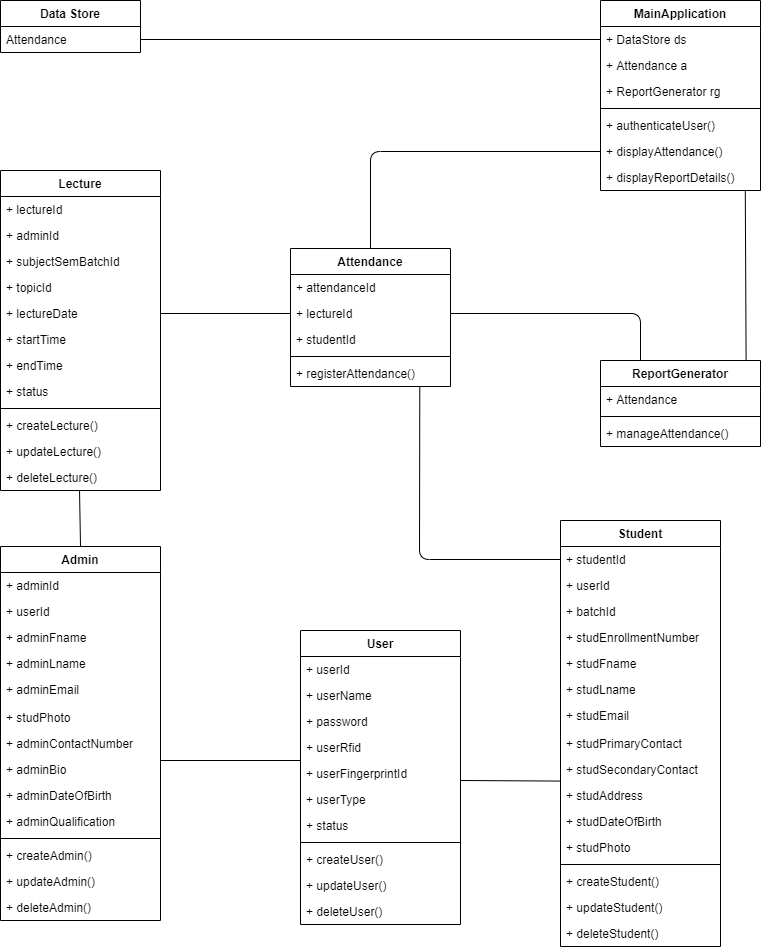
\includegraphics[scale=.5]{Images/uml/Attendance_manage.png}
    \end{center}

\end{enumerate}